%NOTE: texlive ubuntu use pdflatex -shell-escape sprava.tex

\documentclass[12pt,a4paper]{article}

\usepackage[slovak]{babel}
\usepackage[utf8]{inputenc}
\usepackage{listings}
\usepackage{graphicx}
\usepackage{tabularx} 
\usepackage{amsmath} 
\usepackage{amssymb} 
\usepackage{hyperref} 
\usepackage{multicol} 

\usepackage{epstopdf} 
\linespread{1.5}

\lstset{
language=python
,breaklines=true
,basicstyle=\ttfamily
, showstringspaces=false}

\textwidth 6.5in
\oddsidemargin 0.0in
\evensidemargin 0.0in

\begin{document}

\thispagestyle{empty}
\begin{center}
    \large{
        \textbf{
            UNIVERZITA KOMENSKÉHO V BRATISLAVE \\ 
            FAKULTA MATEMATIKY, FYZIKY A INFORMATIKY
        }
    }
\end{center}

\vspace{2cm}

\begin{figure}[!h]
    \centering
    
\includegraphics[width=3.5cm]{komlogo-new.pdf}
\end{figure}

\vspace{1cm}

\begin{center}
    \large{
        \textbf{
            ANALÝZA A RIEŠENIA PROBLÉMOV PORTÁLU data.gov.sk
        }\\
        
        2-INF-106	Informatika a spoločnosť \\
        (Seminárna práca)\\ 
        \href{https://github.com/koniiiik/opendata-sk-ias}{https://github.com/koniiiik/opendata-sk-ias} 
            
        \vspace{1.5cm}
        
        \textbf{
            Peter Csiba, Eduard Eiben, \\  
            Martin Kolínek, Michal Petrucha
        } \\
            %Analýza algoritmov učenia na báze zovšeobecnenej recirkulácie v obojsmerných neurónových sieťach

    }
\end{center}

\vfill

\begin{multicols}{2}
    \begin{flushleft}
        \textbf{23.5.2014}
    \end{flushleft}
    \begin{flushright}
        \textbf{Bratislava}
    \end{flushright}
\end{multicols}

\newpage

\section{Úvod}

Data.gov.sk, ďalej len {\bf portál}, je snahou o implementovanie princípov open data \ref{opendata} v kontexte Slovenskej republiky. Open data je rozširujúci sa koncept silno podporovaný Európskou úniou. Slovensko je vzhľadom na západné krajiny v tomto smere pozadu. Napr. Veľká Británia zverejňuje veľké množstvo dát automatizovane na týždennej báze. Viac o open data v časti \ref{opendata}. 

\subsection{Cieľ práce}
Našou prácou je zmysluplne pomôcť portálu data.gov.sk. Jedným z problémov sú manuálne úkony na portáli. Ako programátori sa preto snažíme automatizovať časť procesov. Hlavnými dvoma procesmi sú automatická kontrola kvality dát.% a automatické získavanie relevantných datasetov, ktoré popisuje v časti \ref{problem-statement}. 

\section{Postup práce}
Naša práca sa dá rozdeliť na dve časti. Prvou časťou bola \emph{analýza} problému, ktorý sme potom riešili \emph{implementáciou}. 

\subsection{Komunikácia}
Aby sme sa v tematike zorientovali, tak sme komunikovali s relevantnými subjektmi, ktoré sa problematikou priamo alebo nepriamo zaoberajú. 

\begin{itemize} 
  \item Úrad splnomocnenca vlády SR pre rozvoj občianskej spoločnosti - \emph{správca portálu} data.gov.sk. 
  \item Aliancia Fair Play - zverejňujú verejné štátne dáta na ich portály datanest (\cite{datanest}), ktoré sú vhodné pre poukázanie korupcie verejných činiteľov. 
  \item OpenData.sk (\cite{opendata-sk}) - zaoberajú sa podobnou problematikou ako data.gov.sk. 
  \item Foaf.sk a Minio.sk - poskytujú jednoduché rozhranie pre verejné štátne dáta, ktoré je efektívne použiteľné.  
\end{itemize} 

\subsection{Stav portálu data.gov.sk} 
Po komunikácií a vlastnej analýze sme dospeli k záveru, že rozsah aj kvalita dát portálu sú značne obmedzené. K podobnému záveru prišli aj ďalšie pracovné skupiny, ktorých výsledky sú zverejnené na portáli opendata.sk. Navrhujú riešenia, ale bohužiaľ, zatiaľ nevidíme ich realizáciu. Dôvody nedostatkov sú rôzne. Za hlavný dôvod považujeme, že napriek mnohým infožiadostiam o zverejnenie dát štátne subjekty nie sú ochotné tieto dáta zverejniť. V tomto vidíme priestor na potenciálne zlepšenie. 

Napríklad AFP získala užitočné datasety pomocou opakovaných infožiadostí, využijúc infozákon, podľa ktoré sú štátne inštitúcie povinné zverejniť viaceré dáta. Avšak kým občanom nechýbajú, tak si inštitúcie nebudú vyrábať prácu navyše. Druhým príkladom spracovania verejných dát sú projekty foaf.sk a finstat.sk, ktorý vyriešili dostupnosť a spracovateľnosť verejných dát ich automatizovaným stiahnutím, offline spracovaním a ich zverejnením v jednoduchšej podobe spolu s relevantnými štatistikami. 

\subsection{Formulácia problému} 
\label{problem-statement}

Vzhľadom na obmedzený rozsah nášho projektu a prakticky neobmedzený rozsah práce na portáli sme boli nútení si vybrať časť na ktorej budeme pracovať. Ostatné nápady sú popísané v časti \ref{future-work}. 

Vychádzali sme z dokumentu \cite{525} vypracovaným skupinou opendata.sk, ktorý obsahuje zoznam 525 datasetov, ktoré by bolo \emph{užitočné} zverejniť. Zvolili sme nasledovný postup:  
\begin{itemize} 
\item Exportovať zoznam do SQL DB a vyčistiť ho. 
\item Previazať databázu s data.gov.sk a zistiť, ktoré datasety už sú získané. 
\item Previazať s výsledkami manuálnej kontroly data.gov.sk z marca 2014. 
\item Zautomatizovať manuálnu kontrolu z predošlého bodu, t.j. či sú odkazy na dáta platné, aké majú chyby a tak ďalej. Inšpirovali sme sa jednoduchým skriptom od \cite{hany}. 
\item Implementovať \emph{5-star} (\cite{5star}) rating kvality datasetov. Podobná funkcionalita existuje v plugine \emph{ckanext-qa} pre CKAN, systém používaný data.gov.sk pre zverejnenie open data.  
\end{itemize} 

\subsection{Implementácia}

Najprv sme skonvertovali zoznam 525 užitočných datasetov do SQLite databázy $D$, ktorú sme následne prečistili. Napr. opravili niektoré preklepy, aby boli dva sémanticky ekvivalentné hodnoty rovnaké aj syntakticky. 

Ďalej sme využili CKAN REST API, aby sme získali aktuálny stav data.gov.sk. Vychádzajúc z API a databázy $D$ sme implementovali nasledovné dva skripty. 

\paragraph{check.py}
Portál data.gov.sk obsahuje iba odkazy na datasety a preto je nutné kontrolovať, či sú odkazy platné. V tomto skripte k danému datasetu získame všetky odkazy a HTTP-requestom overíme, či dataset naozaj existuje. Navyše kontrolujeme hlavičky HTTP-requestu a snažíme sa uhádnuť reálnu príponu súboru, ktorá sa môže líšiť od prípony v URL adrese. Ďalej sa snažíme zistiť, či išlo o presmerovanie a či stránka obsahuje formulár, ktorý je rozhraním pre dataset. Na základe týchto údajov aproximujeme kvalitu datasetu podľa štandardu popísaného v časti \ref{zakon-kvalita}. 

\paragraph{vyhladavac.py} 
Tento čiastočne automatický skript sa snaží prepojiť záznamy databázy $D$ so záznamami na data.gov.sk. Pre každý záznam databázy $D$ vyhľadá skript pomocou CKAN REST API datasety s podobným názvom. V prípade, že výsledkov je viacero, tak skript ponúkne užívateľovi na výber všetky možnosti. Tieto prepojenia sú ukladané do našej databázy $D$. 

%Niekedy sa stane, že v CKANe daný dataset skutočne je, ale skript ho nenájde. Napr. môže byť rozdelený na viacero CKANových datasetov. Takéto prípady sme označili za neexistujúce a zapísali do \href{https://github.com/koniiiik/opendata-sk-ias/blob/master/problematicke_id}{problematicke\_id} spolu s popisom, čo sa pokazilo. Tieto prípady sa dajú vyriešiť aj ručne keďže ich je pomerne málo. Nakoniec sme sa neexistujúce prípady snažili priradiť ručne. Z databázy zaujímavých sme zistili pod ktoré ministerstvo patria a použili ako filter na data.gov.sk.
%CKAN query language Shit => "-slovo" = neobsahuje slovo

Zaujímavosťou boli problémy s názvami datasetov. Napr. dvakrát sa stalo, že bolo viacero datasetov, ktorých názvy sa líšili iba v posledných pár slovách a CKAN search na jeden dataset vrátil všetky okrem toho hľadaného\footnote{
Napr. dvojica 313, 314 a jedna trojica 1716, 1717, 1718.
}. Alebo niektoré datasety mali rozdielne názvy na data.gov.sk a v databáze $D$, napriek tomu, že význam bol ten istý. 

\section{Výsledky}

V tejto časti prezentujeme niektoré vlastnosti datasetov z \cite{525}. Pre každý dataset z tohto zdroja je známe, či je zo zákona zverejniteľný a či rezort súhlasí s jeho zverejnením.

Datasety verejnej správy, ktoré poskytli jednotliví prevádzkovatelia majú rôzne formáty. Obrázok \ref{formaty} ukazuje zastúpenie jednotlivých formátov vo zverejniteľných datasetoch. Dá sa vidieť, že najväčší podiel na zverejniteľných datasetoch majú tabuľky programu Microsoft Excel. Nasledujú databázy rôznych druhov, pdf dokumenty a dokumenty programu Microsoft Word. 

\begin{figure}
\center 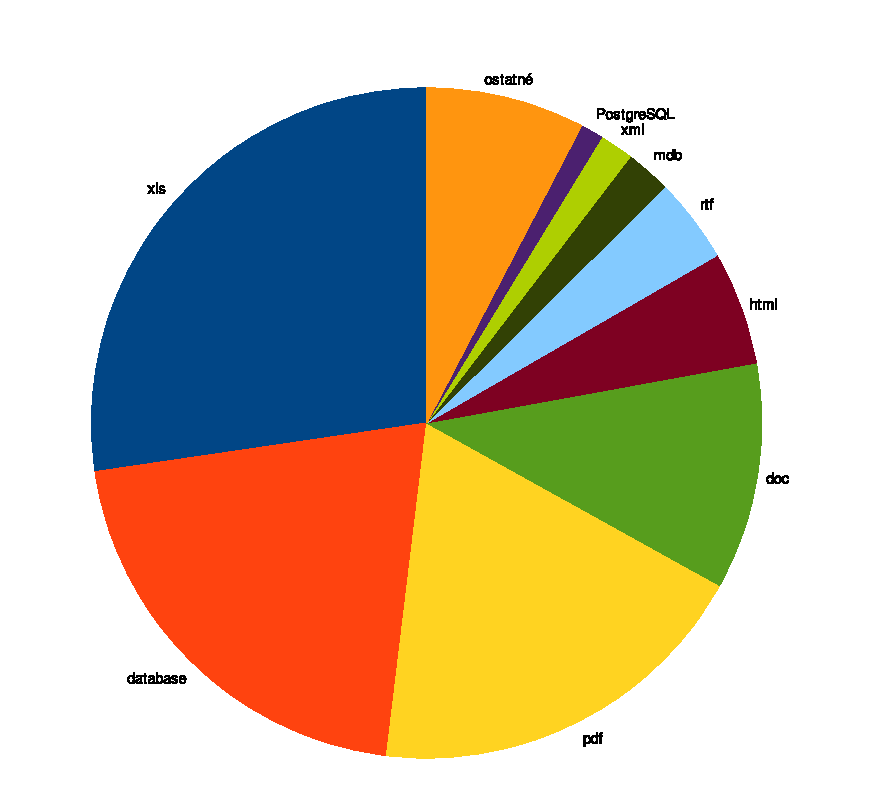
\includegraphics[width=9cm]{dataset_formaty}
\caption{Zastúpenie jednotlivých formátov medzi zverejniteľnými datasetmi, s ktorých zverejnením rezorty súhlasili.}
\label{formaty}
\end{figure}

Ďalej ukážeme, ako je na tom zverejňovanie datasetov pre jednotlivých prevádzkovateľov. Obrázok \ref{zverejnene} ukazuje, aká časť zverejniteľných datasetov, s ktorých zverejnením rezort súhlasil, je zverejnená na data.gov.sk. Dá sa vidieť, že väčšina prevádzkovateľov súhlasila so zverejnením viacerých datasetov ako je naozaj zverejnených.

\begin{figure}
\center 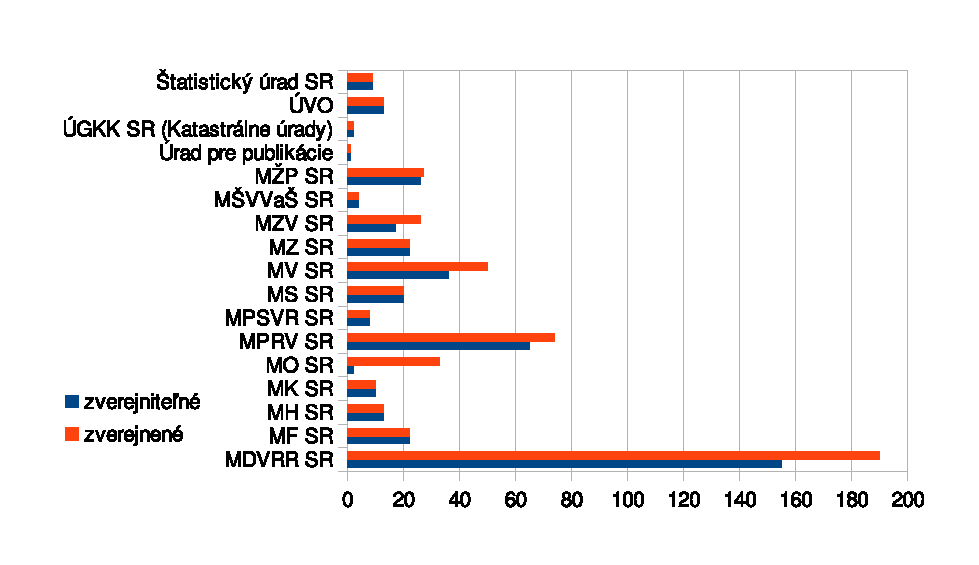
\includegraphics[width=14cm]{zverejnene_prevadzkovatel}
\caption{Zverejnené a zverejniteľné datasety pre jednotlivých prevádzkovateľov.}
\label{zverejnene}
\end{figure}

Pri hľadaní dôvodu sme sa pozreli na formáty zverejniteľných, ale ešte nezverejnených datasetov. Obrázok \ref{nezverejnene_formaty} ukazuje distribúciu jednotlivých formátov. Dá sa vidieť, že medzi nezverejnenými datasetmi je najviac datasetov vo formáte databázy. Predpokladáme, že export dát z databázy v otvorenom formáte často nie je taký jednoduchý.

\begin{figure}
\center 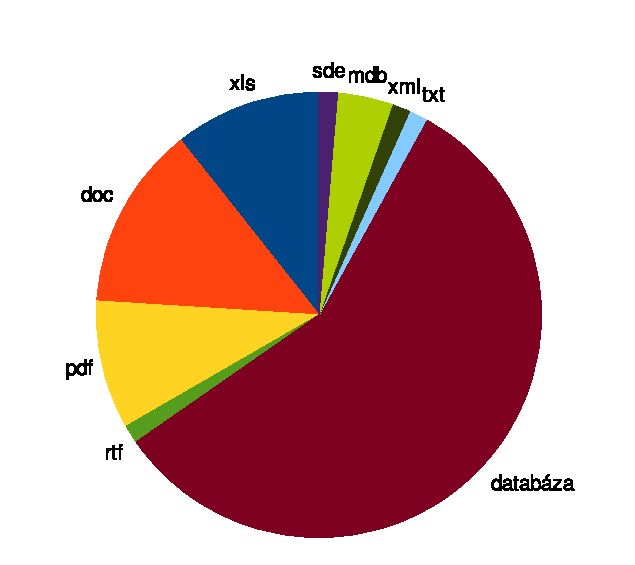
\includegraphics[width=9cm]{nezverejnene_formaty}
\caption{Zastúpenie formátov medzi nezverejnenými, ale zverejniteľnými datasetmi.}
\label{nezverejnene_formaty}
\end{figure}

Na koniec sa pozrieme na stav datasetov zverejnených na data.gov.sk. Obrázok \ref{stars} ukazuje hodnotenie datasetov podľa 5 hviezdičkového hodnotenia z \cite{5star}. Vidíme, že väčšina datasetov má 3 hviezdičky. To značí datasety, ktoré majú otvorený formát a sú štrukturované. Treba ale myslieť na to, že v skutočnosti nemá väčšina datasetov ani jednu hviezdičku, lebo nemajú otvorenú licenciu.

Tiež sa pozrieme na dostupnosť jednotlivých datasetov. Obrázok \ref{status} ukazuje, aký je stav datasetov na data.gov.sk. Vidíme, že väčšina datasetov je v poriadku dostupná. Ale niekoľko datasetov nie je dostupných. Tak isto existujú na data.gov.sk datasety, ktorých zdroj presmeruje na inú stránku. Na obrázku \ref{status} je ukázané, koľko datasetov je prístupných iba po vyplnení webového formulára.

\begin{figure}
\center 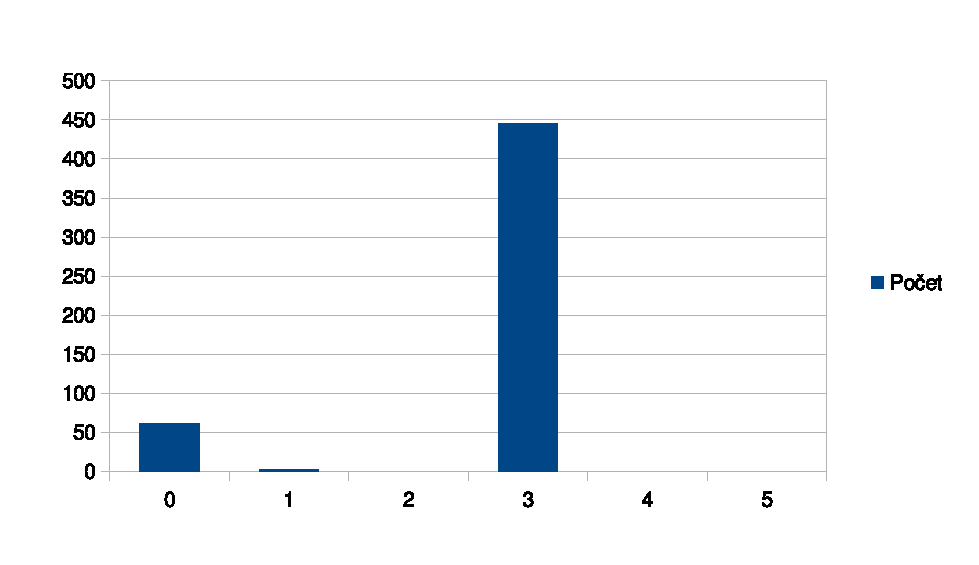
\includegraphics[width=14cm]{stars}
\caption{Počty datasetov pre jednotlivé hodnotenia.}
\label{stars}
\end{figure}

\begin{figure}
\center 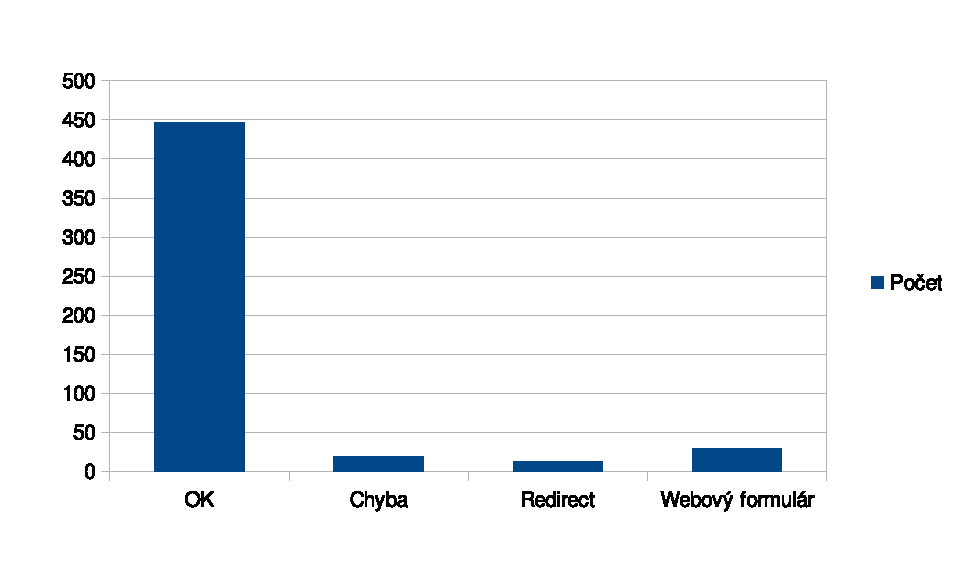
\includegraphics[width=14cm]{status}
\caption{Počty datasetov v jednotlivých stavoch.}
\label{status}
\end{figure}

\section{Záver} 

Previazaním data.gov.sk a zoznamu datasetov užitočných na zverejnenie sme definovali ktoré datasety treba hľadať a žiadať, či už manuálne alebo automaticky. Ďalej sme automatizovali kontrolu kvality a nedostatkov, na ktorom sa dá ďalej stavať. Tento text poskytuje náhľad aktuálneho stavu portálu a jeho problémov. 

\paragraph{Budúca práca.} 
\label{future-work} 
Za hlavné pokračovanie považujeme automatizované vyhľadávanie žiadaných datasetov pomocou vyhľadávačov. V našom repozitáry existuje neúplný zoznam webových stránok štátnych inštitúcií ako aj skript na automatizované parse-ovanie výsledkov vyhľadávania. Navrhujeme pre každú webstránku spustiť vyhľadávanie pre názov a súborovú príponu. 

Ďalším možným pokračovaním by bolo pomáhať štátu zverejňovať tieto dáta. V porovnaní so západnými krajinami tu existuje veľký priestor na zlepšenie. Na druhej strane sú tieto realizácie vhodnou inšpiráciu pre náš štát. Veríme, že vhodnou spoluprácou štátu a skupinami šikovných programátorov je tento výsledok dosiahnuteľný. V každom prípade je to ale beh na dlhé trate. 

\renewcommand{\refname}{Literatúra}
\phantomsection
\addcontentsline{toc}{section}{Literatúra}
\begin{thebibliography}{99}
  \bibitem{proj} \url{https://github.com/koniiiik/opendata-sk-ias} - Repozitár nášho projektu s dokumentáciou. 
  \bibitem{525} \url{http://www.otvorenavlada.gov.sk/datasety-statnej-spravy/} - Zoznam datasetov \emph{užitočných} na zverejnenie.
  \bibitem{hodnotenie} \url{http://www.otvorenavlada.gov.sk/navrh-hodnotiacej-spravy-iniciativy-pre-otvorene-vladnutie-v-slovenskej-republike/} - Návrh hodnotiacej správy Iniciatívy pre otvorené vládnutie v Slovenskej republike.
  \bibitem{kvalita} \url{http://www.zbierka.sk/sk/predpisy/55-2014-z-z.p-35621.pdf} - Výnos 55/2014 aj o kvalite Open data. 
  \bibitem{hany} \url{https://github.com/hanecak/data.gov.sk-link-check/} - Základná kontrola odkazov datasetov portálu CKAN. 
  \bibitem{datanest} \url{http://datanest.fair-play.sk/pages/index} - Datanest Aliancie Fair play. 
  \bibitem{opendata-sk} \url{http://opendata.sk/liferay/studia-open-data-portal} - OpenData.sk. 
  \bibitem{opendata-wiki} \url{http://en.wikipedia.org/wiki/Open_data} - Definícia open data na Wikipédií. 
  \bibitem{5star} \url{http://5stardata.info/} - 5 star hodnotenie. 
\end{thebibliography}


\section*{Príloha - Vysvetlenie pojmov} 
\subsection*{Open data} 
\label{opendata} 
Open data je myšlienka, že niektoré dáta by mali byť dostupné pre každého na akékoľvek použitie, bez akýchkoľvek licencií, patentov alebo iných kontrolných mechanizmov. Ciele open data sú podobné ako iných \emph{otvorených} spoločností, ako sú open source, open hardware a iné. Filozofia open data je stará ale termín \emph{open data} je súčasný a naberá na popularite s rastom Internetu a WWW. Najpokročilejšími portálmi sú data.gov a data.gov.uk (\cite{opendata-wiki}). 

\subsection*{Hodnotenie kvality datasetov}
\label{zakon-kvalita} 
Kvalitu dát sme hodnotili podľa \emph{výnosu 55/2014} (\cite{kvalita}) popisujúci aj \emph{kvalitu datasetu poskytovaného povinnou osobou}, ktoré vychádza z hodnotenia 5 star (\cite{5star}) a je rozdelené na šesť úrovní: 
\begin{itemize} 
\item úroveň 0, pri ktorej nie je dataset poskytovaný
v elektronickej forme,
\item úroveň 1, pri ktorej je dataset dostupný vo webovom
prostredí,
\item úroveň 2, pri ktorej je splnená požiadavka uvedená
v písmene b) a obsah datasetu je štruktúrovaný tak,
že umožňuje automatizované spracovanie,
\item úroveň 3, pri ktorej sú splnené požiadavky uvedené
v písmene c) a dataset je poskytovaný v otvorenom
formáte, nezávislom na konkrétnom proprietárnom
softvéri,
\item úroveň 4, pri ktorej sú splnené požiadavky uvedené
v písmene d) a na identifikáciu údajov datasetu a ich
vzťahov sa používajú refencovateľné identifikátory,
\item úroveň 5, pri ktorej sú splnené požiadavky uvedené
v písmene e) a dataset a jeho interné a externé
vzťahy majú charakter identifikátormi prepojených
údajov.
\end{itemize} 

Ak sa údaje poskytujú pre automatizované spracovanie, štandardom kvality datasetu poskytovaného
povinnou osobou je aj ich poskytovanie ako datasetu s otvorenými údajmi podľa § 53 a v kvalite najmenej úrovne 3.


\end{document} 
